\documentclass[12pt, letterpaper, twoside]{article}
\usepackage{nopageno,epsfig, amsmath, amssymb}
\usepackage{physics}
\usepackage{mathtools}
\usepackage{hyperref}
\usepackage{xcolor}
\hypersetup{
    colorlinks,
    linkcolor={blue},
    citecolor={blue},
    urlcolor={blue}
}
\usepackage{empheq}
\usepackage{wrapfig}

\usepackage[letterpaper,
            margin=0.8in]{geometry}

\newcommand{\psetnum}{1}
\newcommand{\class}{ASTR 558 - Exoplanets}

\newcommand{\tomtitle}{
    \noindent {\LARGE \fontfamily{cmr}\selectfont \textbf{\class}} \hfill \\[1\baselineskip]
    \noindent {\large \fontfamily{cmr}\selectfont Problem Set \psetnum \hfill \textsc{Tom Wagg}}\\[0.5\baselineskip]
    {\fontfamily{cmr}\selectfont \textit{\today}}\\[2\baselineskip]
}

\title{\class : Problem Set \psetnum}
\author{\textbf{Tom Wagg}}

\newcommand{\question}[1]{{\noindent \it #1}}
\newcommand{\answer}[1]{
    \par\noindent\rule{\textwidth}{0.4pt}#1\vspace{0.5cm}
}
\newcommand{\todo}[1]{{\color{red}\begin{center}TODO: #1\end{center}}}

% custom function for adding units
\makeatletter
\newcommand{\unit}[1]{%
    \,\mathrm{#1}\checknextarg}
\newcommand{\checknextarg}{\@ifnextchar\bgroup{\gobblenextarg}{}}
\newcommand{\gobblenextarg}[1]{\,\mathrm{#1}\@ifnextchar\bgroup{\gobblenextarg}{}}
\makeatother

\newcommand{\avg}[1]{\left\langle #1 \right\rangle}
\newcommand{\angstrom}{\mbox{\normalfont\AA}}
\allowdisplaybreaks

\begin{document}

\tomtitle

\noindent All code that I used for this homework can be found in \href{https://www.github.com/TomWagg/uw-grad-classes/blob/main/558_exoplanets/pset1/planet_finder.py}{\texttt{planet\_finder.py}}. Just run \texttt{python planet\_finder.py} to reproduce all results. \\

\question{\textbf{Q1. Kepler Solver}}
\answer{
    I wrote a solver for Kepler's equation in the function \texttt{solve\_kepler\_equation()} and validated it in \texttt{test\_kepler\_solver()} by putting the resulting eccentric anomalies back into the Kepler equation and checking that the equation still holds.
}

\question{\textbf{Q2. Radial Velocity Equation}}
\answer{
    This is implemented in \texttt{radial\_velocity()}. It is formulated slightly differently from class because I figured I could simplify some of the trig and write the formula instead as the following by using the addition identities.
    \begin{equation}
        v_{rv} = k_* \qty[ \cos (f(t) + \omega) + e \cos \omega ] + \gamma
    \end{equation}
    \vspace{-1cm}
}

\question{\textbf{Q3. Find planet period}}
\answer{
    I followed the method that Eric demonstrated in class in order to find the period. I chose a grid of periods over which to search and, for each of them, folded the data based on this period, sorted it by phase and then calculate the sum of the square of the difference between adjacent points. I plot this in a periodogram in the figure below.

    \begin{center}
        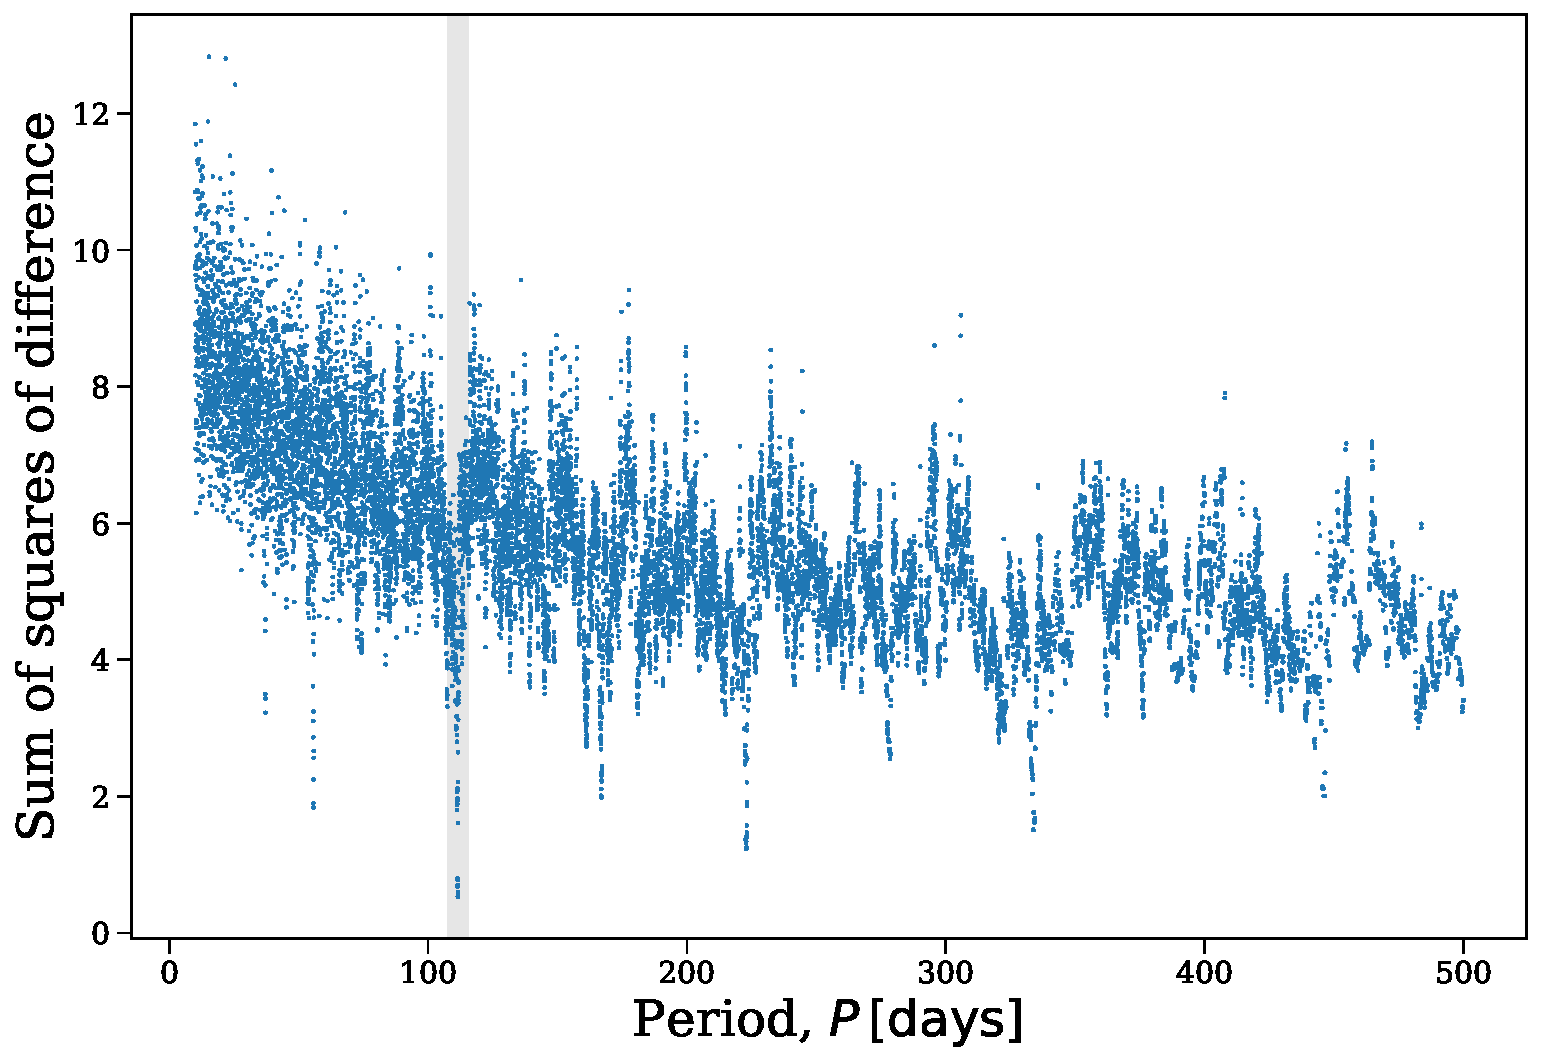
\includegraphics[width=0.55\textwidth]{figures/periodogram.pdf}
    \end{center}
    The minimum of this plot should give the period (which I highlight with a grey bar) and so I find that the period of the planet is
    \begin{equation}
        \boxed{ P = 111.47 \unit{days} }
    \end{equation}
}

\question{\textbf{4. Fit planet parameters}}
\answer{
    Now for the main event! I fitted for the planet parameters $(P, k_*, t_p, \gamma, \omega, e)$ using \texttt{emcee}. I set the initial guess for $P$ using the answer from Q3. For $k_*$ I used $0.5(v_{rv, {\rm max}} - v_{rv, {\rm min}})$ from the definition. I guessed values for the other four just by playing around with them until the fit looked sort of close. This gave initial guesses as
    \begin{equation}
        \mathrm{initial\ guesses} = [111.47 \unit{days}, 0.4973 \unit{km}{s^{-1}}, 10.7 \unit{days}, -0.1 \unit{km}{s^{-1}}, 5 \unit{rad}, 0.92]
    \end{equation}
    for $P, k_*, t_p, \gamma, \omega, e$ respectively. I then applied the following bounds as a prior
    \begin{equation}
        \begin{split}
            \mathrm{bounds} =
                [&(110, 112) \unit{days}, (0.2, 0.7) \unit{km}{s^{-1}}, (10.2, 11.2) \unit{days},\\
                &(-1, 1) \unit{km}{s^{-1}}, (0.01, 2 \pi) \unit{rad}, (0, 1)]
        \end{split}
    \end{equation}
    Next I ran \texttt{emcee} using 16 walkers, with 5000 steps each and a 1000 step burn in. I've plotted the parameter distribution as a corner plot and \textbf{I put it at the end of this document}.
    
    There are some interesting correlations. The one between $P$ and $t_p$ makes a lot of sense, if the period is longer then the sharp transition is also going to move. I'm less confident about the reasoning behind the correlations between $e$ and $k_*$ plus $\gamma$ but I \textit{think} this is because all of these parameters each tend to `stretch' the model in radial velocity and so they tend to have interdependencies?

    To get the best fit for the parameters, I take the median values from each of these distributions. The best fit values are:
    \begin{equation}
        \boxed{ P, k_*, t_p, \gamma, \omega, e = 111.31 \unit{days}, 0.471 \unit{km}{s^{-1}}, 10.92 \unit{days}, -0.0019 \unit{km}{s^{-1}}, 5.251 \unit{rad}, 0.932}
    \end{equation}
    I plot this with the folded data (on the same period as the fit) in the plot below - and it shows that we have good agreement, fun!
    \begin{center}
        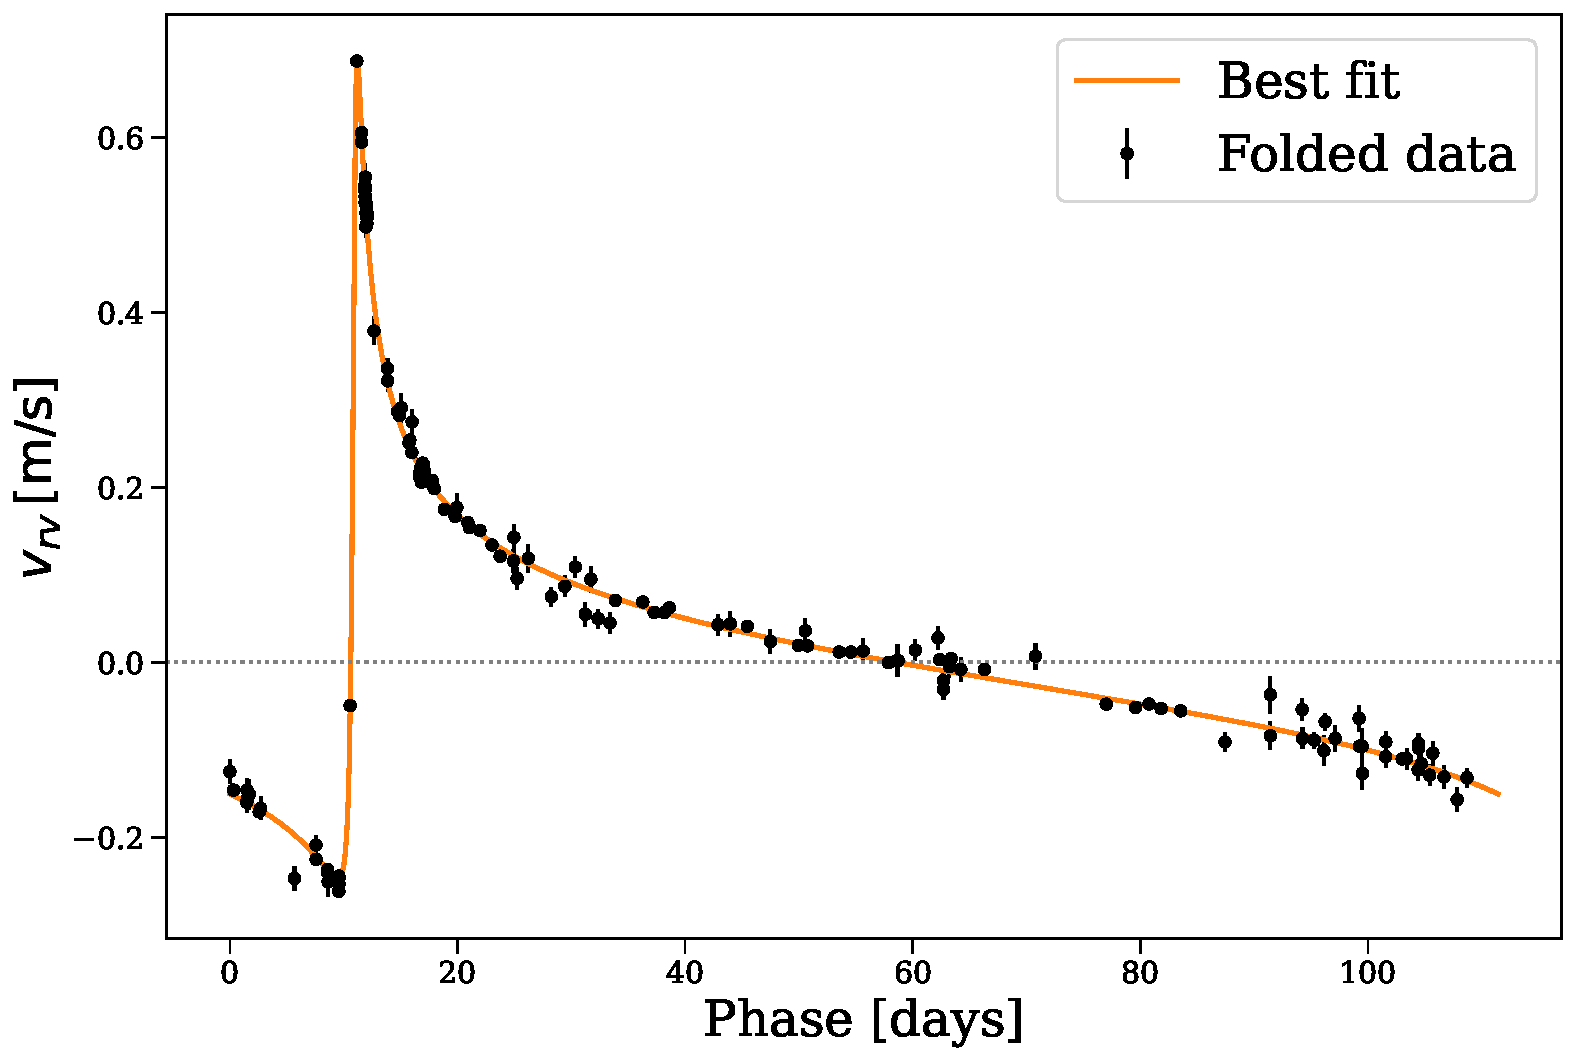
\includegraphics[width=0.8\textwidth]{figures/best_fit.pdf}
    \end{center}
    So now I got intrigued and wondered what this meant for the mass of the planet. Since we know that $k_*$ is defined as
    \begin{equation}
        k_* = \qty(\frac{2 \pi G}{P (1 - e^2)})^{1/3} \frac{M_p \sin \iota}{(M_* + M_p)^{2/3}},
    \end{equation}
    where $\iota$ is the inclination and $M_*$ is the star mass. It should be fairly reasonable to rearrange this to find the planet mass and make the assumption that $M_* \gg M_p$ (this worries me slightly but I figure it'll be fine except in extreme cases). This gives that the planet mass is
    \begin{equation}
        M_p = \frac{k_* M_*^{2/3}}{\sin \iota} \qty(\frac{2 \pi G}{P (1 - e^2)})^{-1/3},
    \end{equation}
    So now we know everything in this equation from the best fit except $\iota$ and $M_*$. I made a grid of these values and plotted the planet mass as a contour plot below along with some lines indicating Saturn, Jupiter and Kepler-25b (one of the most massive planets found).

    \begin{center}
        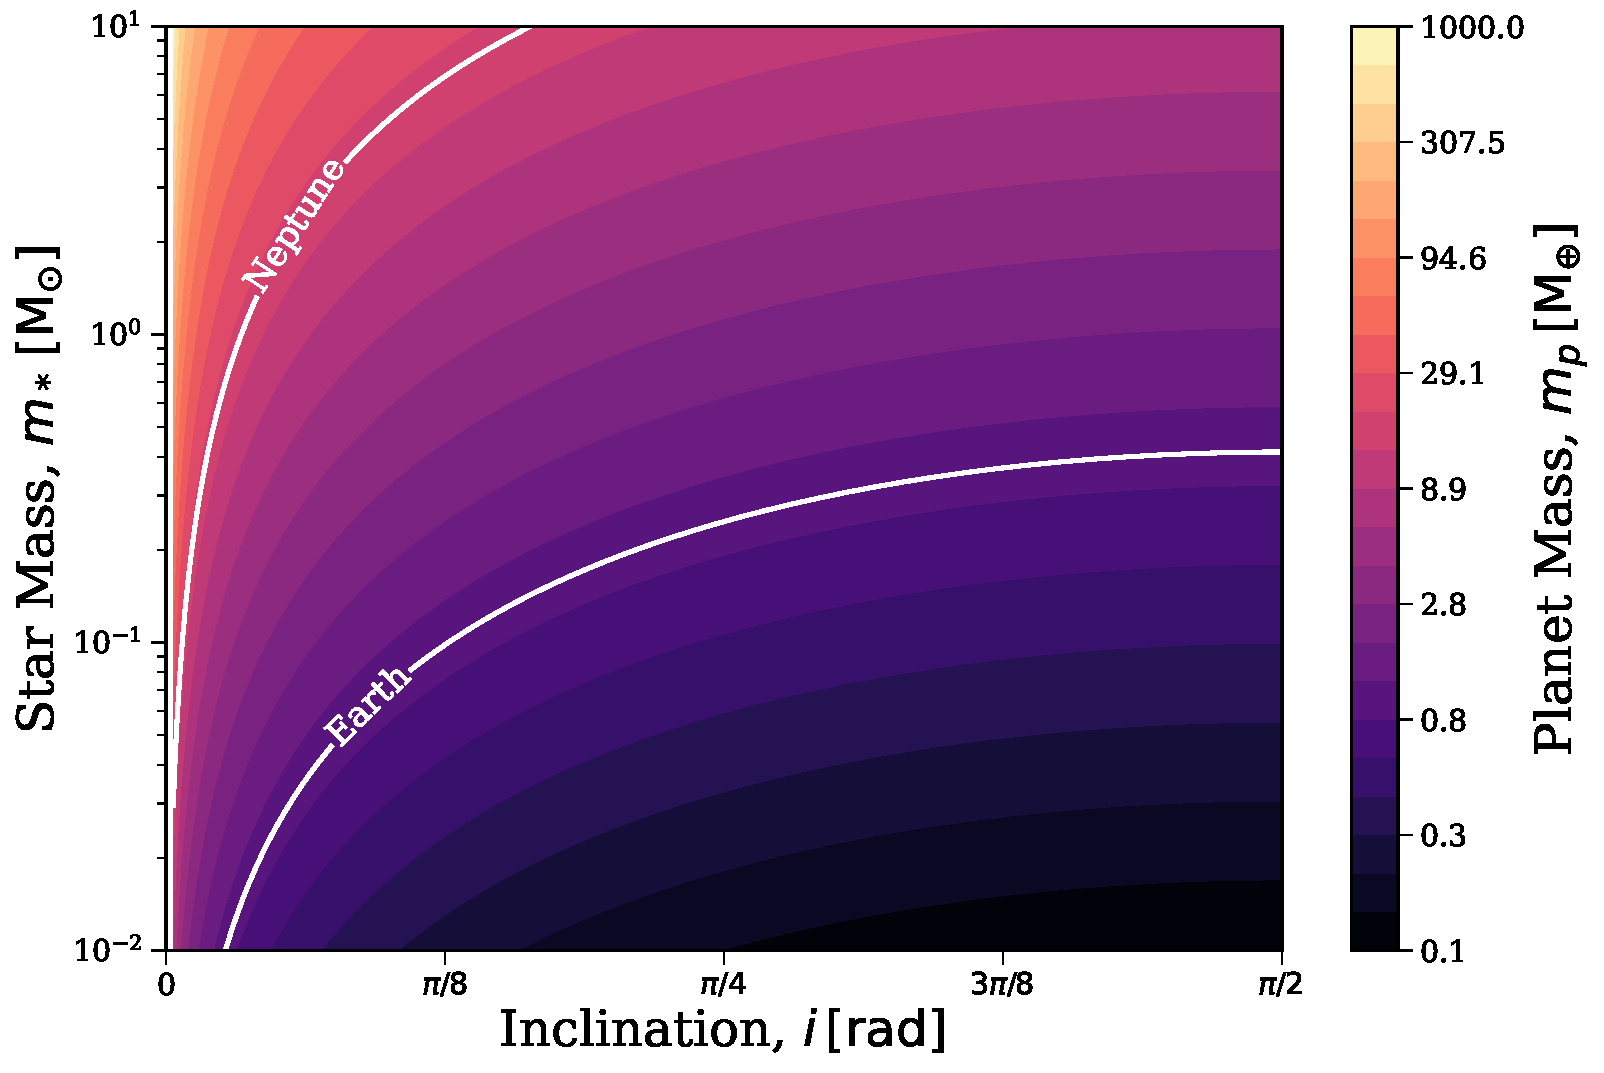
\includegraphics[width=\textwidth]{figures/planet_mass.pdf}
    \end{center}

    After some quick googling of the parameters that I found, it looks like our mystery planet is none other than HD 80606b! In this case, I can use the values of $M_* = 0.98 \pm 0.1 \unit{M_\odot}$ and $\iota = 89.6 \pm 0.4$ from \href{https://arxiv.org/abs/0902.4457}{Table 1 of this paper} (shown as black point with errorbars on plot). Plugging these into the equation above give that the mass of the planet should be
    \begin{equation}
        M_p \approx 5.59 \unit{M_{\rm Jup}}
    \end{equation}
    The real answer is $4.0 \pm 0.3 \unit{M_{\rm Jup}}$...but that's not far off given this is the most basic fit I could come up with in just a couple of hours, very fun! :D
}

\clearpage

\question{\textbf{6. Gauss Functions}}

\question{Part a - Conservation of Angular Momentum}
\answer{
    We are given that the Gauss functions are defined such that
    \begin{align}
        \va{x} &= f \va{x}_0 + g \va{v}_0 \\
        \va{v} &= \dot{f} \va{x}_0 + \dot{g} \va{v}_0
    \end{align}
    Let's use these to show that when angular momentum is conserved then the relation given holds. If angular momentum is conserved then it must be the case that
    \begin{equation}
        \va{x}_0 \cross \va{v}_0 = \va{x} \cross \va{v}
    \end{equation}
    We can now apply the fact that the cross product is distributive and the following identities
    \begin{align}
        \va{a} \cross \va{a} &= 0, \\
        \va{a} \cross \va{b} &= - \va{b} \cross \va{a},
    \end{align}
    to the conservation equation to show the required relation.
    \begin{align}
        \va{x}_0 \cross \va{v}_0 &= \va{x} \cross \va{v} \\
                                 &= \qty(f \va{x}_0 + g \va{v}_0) \cross (\dot{f} \va{x}_0 + \dot{g} \va{v}_0) \\
                                 &= (f \dot{f}) (\va{x}_0 \cross \va{x}_0) + (f \dot{g}) (\va{x}_0 \cross \va{v}_0) + (g \dot{f}) (\va{v}_0 \cross \va{x}_0) (g \dot{g}) (\va{v}_0 \cross \va{v}_0) \\
                                 &= (f \dot{g}) (\va{x}_0 \cross \va{v}_0) - (g \dot{f}) (\va{x}_0 \cross \va{v}_0) \\
        \va{x}_0 \cross \va{v}_0 &= (f \dot{g} - g \dot{f}) (\va{x}_0 \cross \va{v}_0) \\
                               \Aboxed{ \implies 1 &= f \dot{g} - g \dot{f} }
    \end{align}
}

\question{Part b - Kepler's Equation Satisfied}
\answer{
    Right then, let's get into the weeds! We are given that the Gauss functions are
    \begin{align}
        f &= \frac{a}{r_0} \qty(\cos (E - E_0) - 1) + 1 \\
        g &= (t - t_0) + \frac{1}{n} \qty(\sin(E - E_0) - (E - E_0)) \\
        \dot{f} &= -\frac{a^2}{r r_0} n \sin (E - E_0) \\
        \dot{g} &= \frac{a}{r} \qty(\cos (E - E_0) - 1) + 1
    \end{align}
    We can write these in a nicer form by assuming that $E_0 = M_0 = 0$ and $M = n (t - t_0)$.
    \begin{align}
        f &= \frac{a}{r_0} \qty(\cos E - 1) + 1 \\
        g &= \frac{1}{n} \qty(M + \sin E - E) \\
        \dot{f} &= -\frac{a^2}{r r_0} n \sin E \\
        \dot{g} &= \frac{a}{r} \qty(\cos E - 1) + 1
    \end{align}
    It will also be useful to apply
    \begin{align}
        M &= E - e \sin E \\
        r &= a (1 - e \cos E) \\
        r_0 &= a (1 - e)
    \end{align}
    And now we just plug the whole gaggle of equations into our relation from the previous question
    \begin{align}
        f \dot{g} - g \dot{f} &= \qty[\frac{a}{r_0} \qty(\cos E - 1) + 1] \qty[\frac{a}{r} \qty(\cos E - 1) + 1] - \qty[\frac{1}{n} \qty(M + \sin E - E)] \qty[-\frac{a^2}{r r_0} n \sin E] \\
        &= \frac{a^2}{r r_0} \qty[ \qty(\qty(\cos E - 1) + \frac{r_0}{a}) \qty(\qty(\cos E - 1) + \frac{r}{a}) + \sin E \qty(M + \sin E - E)] \\
        &= \frac{a^2}{r r_0} \qty[ \qty(\cos E - 1 + 1 - e) \qty(\cos E - 1 + 1 - e \cos E) + \sin E \qty(M + \sin E - E)] \\
        &= \frac{a^2}{r r_0} \qty[ \qty(\cos E - e) \qty(\cos E - e \cos E) + \sin E \qty(\sin E - e \sin E)] \\
        &= \frac{a^2}{r r_0} (1 - e) \qty[ \qty(\cos E - e) \cos E + \sin^2 E] \\
        &= \frac{a^2}{r r_0} (1 - e) \qty[ (1 - e \cos E) (\cos^2 E + \sin^2 E)] \\
        &= \frac{a^2}{r r_0} (1 - e) (1 - e \cos E) \\
        &= \frac{a^2}{r r_0} \frac{r_0}{a} \frac{r}{a} \\
        \Aboxed{ f \dot{g} - g \dot{f}&= 1 }
    \end{align}
}

\clearpage

\begin{center}
    \section*{MCMC Corner Plot of Planet Parameters}
    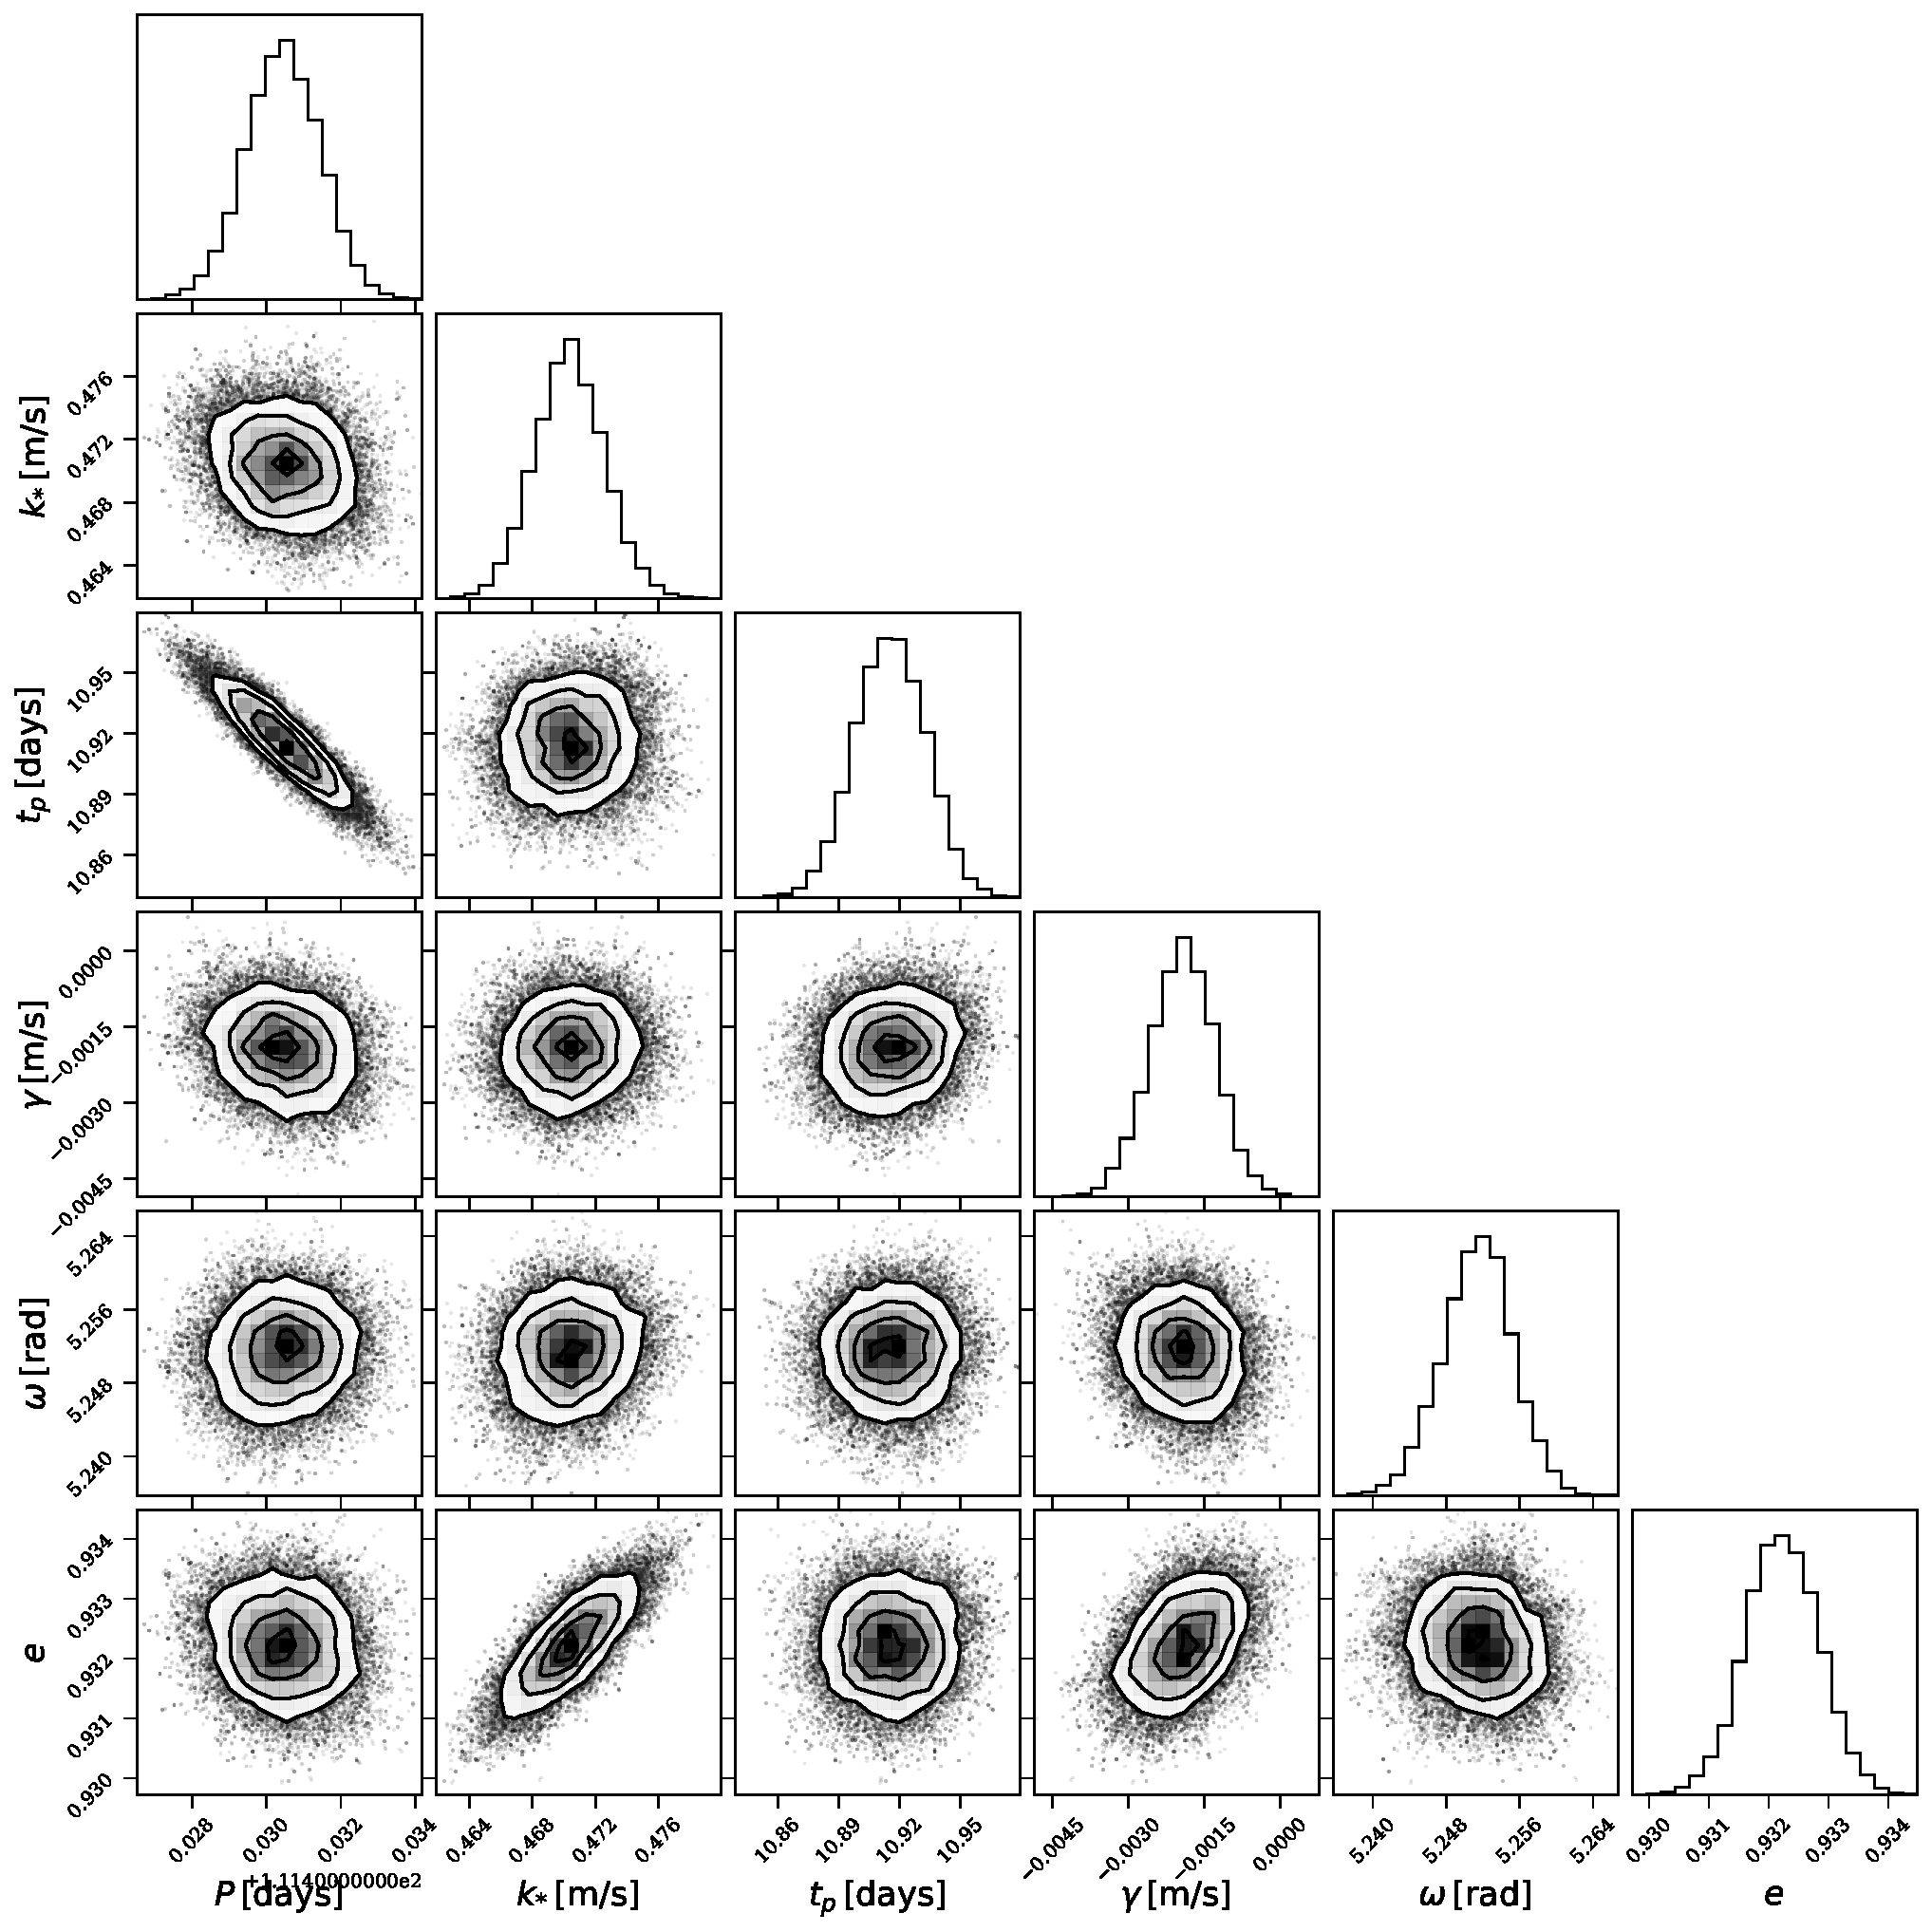
\includegraphics[width=\textwidth]{figures/mcmc_corner.pdf}
\end{center}


\end{document}

 